%%%%%%%%%%%%%%%%%%%%%%%%%%%%%%%%%%%%%%%%%%%%%%%%%%%%%%%%%%%%%%%%%%%%%%%%%%%%%
%%% A Dependency Network+Weigthed Kernel Approach for Feature Selection
%%% Proposal for a MSc Project
%%% Nestor Rodriguez + Sergio A. Rojas (c) 2010
%%%
%%% Chapter 3: Acknowledgements
%%%%%%%%%%%%%%%%%%%%%%%%%%%%%%%%%%%%%%%%%%%%%%%%%%%%%%%%%%%%%%%%%%%%%%%%%%%%%

\section{Idea and Proposal}
\label{sec:IdAndProp}

The new FSS method will involve the following main components (see Figure \ref{fig:im02}). The \emph{data}, which is the sample of observed variables for a given problem; the overall goal of the method will be to identify relevant feature subsets and as much as possible information about dependencies that explain significant patterns hidden in the data.  The \emph{dependency network model} represents the relationships among variables and how they affect each others.  

\begin{figure}[ht]
	\centering
		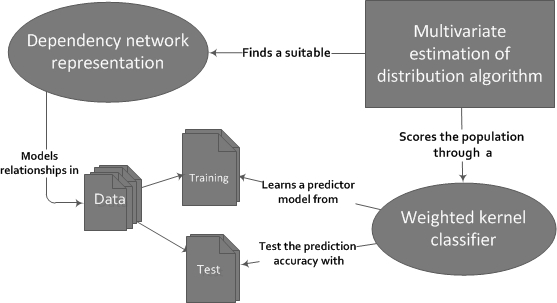
\includegraphics{Images/components.jpg}
	\caption{The components involved in this thesis proposal.}
	\label{fig:im02}
\end{figure}

The \emph{multivariate estimation of distribution algorithm} is a technique to infer the parameters and structure of the dependency network by estimating a probability distribution of relevancy from a pool of candidate weight vectors; the distribution and candidates are adjusted within a framework of a stochastic population-based evolutionary algorithm. Lastly, the \emph{weighted kernel classifier} will perform the iterative classification using relevant feature subsets according to the evolved relevance distributions.

A draft schematic flowchart of the conceived method is shown in Figure \ref{fig:im03}. Preliminary pseudo-code of the method is summarized in Algorithm \ref{alg:idea}.

\begin{figure}[ht]
	\centering
		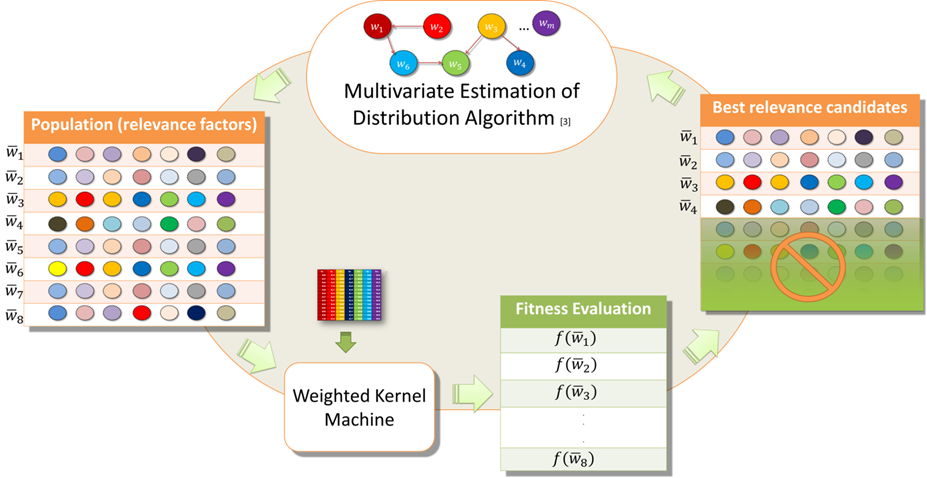
\includegraphics{Images/flowchart.png}
	\caption{Preliminary depiction of the expected method described in this proposal.}
	\label{fig:im03}
\end{figure}

\begin{algorithm}[ht]
	\caption{\textsf{Preliminary pseudocode of the expected method described in this proposal}}
	\begin{algorithmic}
		\REQUIRE Given a dataset $\cD$, a weighted kernel $\kappa_\omega$ and a classifier $\cA$
		\STATE Let $\beta$ represents a dependency network distribution initialized with an independent joint distribution.
		\REPEAT 
			\STATE Split $\cD$ in training $\cD_{t}$ and testing $\cD_{s}$ data
			\STATE $\bar{\Omega} \gets$ Sample $k$ candidates from $\beta$ \pdfcomment[avatar={reviewer}, id = 7]{In algorithm 1 the first set of k candidates is taken from an empty set} \pdfreply[avatar=me, id= 70, replyto=7]{ \emph{Beta} represents a dependency network distribution. Thus in the first algorithm iteration the k candidates are not sample from an empty set but rather from an independent joint distribution. }
			\FOR{$\bomega_j \in \Omega$}
				\STATE Train classifier: $h_j \gets \cA (\cD_{t}, \kappa_{\omega_j})$
				\STATE Test classifier: $e_j \gets$ error$(h_j, \cD_{s}, \kappa_{\omega_j})$
			\ENDFOR
			\STATE $\bar{\Omega}' \gets$ bestCandidates$(\bar{\Omega},\bar{e})$
			\STATE Re-estimate dependency network: $\beta \gets$ reEstimate$(\bar{\Omega}')$
	\UNTIL $\beta$ has converged or maximum number of iterations reached
	\end{algorithmic}
	\label{alg:idea}
\end{algorithm}